\documentclass[a4paper,10pt]{article}
\usepackage[utf8]{inputenc}
\usepackage[margin=1.5cm, bottom=2cm]{geometry}
\usepackage{fancyhdr}
\usepackage{enumitem}
\usepackage{amsmath}
\usepackage{amssymb}
\usepackage{tikz}
\usetikzlibrary{automata, positioning}
\pagestyle{fancy}
\usepackage[most]{tcolorbox}

\newtcolorbox{osservazioni}{
  colback=gray!8,    % sfondo grigio chiaro
  colframe=white,      % nessun bordo
  arc=2mm,            % angoli smussati
  boxrule=0pt,        % spessore bordo 0
  fontupper=\small,
  left=5mm, right=5mm, top=3mm, bottom=3mm,
  before skip=0pt,   % niente spazio prima
  after skip=30pt     % niente spazio dopo
}
\pagestyle{fancy}


%%%%%%%%%%%%%%%%%%%
\newcommand{\EsercitazioneNum}{02}
\newcommand{\Data}{02/10/2025}
%%%%%%%%%%%%%%%%%%%

% Numero di pagina in basso al centro
\fancyhf{}
\fancyfoot[C] \thepage
\renewcommand{\footrulewidth}{0pt} % niente linea in basso
\renewcommand{\headrulewidth}{0pt} % niente linea in alto

\begin{document}
\footnotesize  % font generale più piccolo

\noindent
\small \textbf{Computabilità, Complessità e Logica - a.a. 2025/26} \hfill \textbf{Esercitazione \EsercitazioneNum} \\[0.2cm]
\scriptsize Matteo Liotta, \texttt{matteo.liotta@studenti.units.it} \hfill \Data \\[0.2cm]

\noindent\makebox[\linewidth]{\rule{\linewidth}{0.4pt}} \\[1cm]


\noindent\Large \textbf{Esercitazione \EsercitazioneNum}: \textit{Macchine a stati finiti e Linguaggi Regolari (cont'd)}\\[0cm]
%\\[0.4cm]
\begin{osservazioni}
    \textbf{Pumping Lemma}\\
    Dato $L$ linguaggio regolare definito su $\Sigma$, $\exists p \in \mathbb{N}$ (i.e. \emph{pumping length}) tale che, per ogni $w \in L$ con $|w|\geq p$, si ammette la scrittura:
    $$w = xyz$$
    con:
    \begin{itemize}
        \item $|xy| \leq p$,
        \item $|y| > 0$,
    \end{itemize}
    per cui $$\forall i \geq 0,\; x y^i z \in L$$
\end{osservazioni}


{\normalsize
\begin{itemize}[label=, leftmargin=0pt]

    \item \textbf{Esercizio 8 (*)}\\ Sia $L$ linguaggio regolare su $\Sigma=\{a,b\}$, tale per cui 
    {\begin{center}
        $L = \{ w \in \Sigma^* \mid w = a^nb^m,\ \ \  n,m\geq0 \}$
    \end{center}} 
    Dimostrare la regolarità o la non regolarità di tale linguaggio.\\[0.1cm]


    \item \textbf{Esercizio 9. (*)}\\ Sia $L$ linguaggio su $\Sigma=\{a,b\}$, tale per cui 
    {\begin{center}
        $L = \{ w \in \Sigma^* \mid w = a^kb^n, k<n, \ \ \ n\geq 0\}$
    \end{center}} 
    Dimostrare la regolarità o la non regolarità di tale linguaggio.\\[0.1cm]

    \item \textbf{Esercizio 10. (**)}\\ Si consideri il linguaggio dell'esercizio 5. \textit{(Esercitazione 01)}. Si provi a confermare analiticamente l'intuizione di non regolarità relativa a tale linguaggio. \\[0.1cm]

    \item \textbf{Esercizio 11 (*)}\\ Sia $L$ linguaggio regolare su $\Sigma=\{a,b,0\}$, tale per cui 
    {\begin{center}
        $L = \{ w \in \Sigma^* \mid w = z00, z \in \Sigma^* \}$
    \end{center}} 
    Dimostrare la regolarità o la non regolarità di tale linguaggio.\\[0.1cm]

    \item \textbf{Esercizio 12. (***)}\\ Sia $L$ linguaggio su $\Sigma=\{a,b\}$, tale per cui 
    {\begin{center}
        $L = \{ w \in \Sigma^* \mid w = a^{2^n}, n\geq 0\}$
    \end{center}} 
    Dimostrare la regolarità o la non regolarità di tale linguaggio.\\[0.1cm]

    
    \vfill
    \noindent\makebox[\linewidth]{\rule{\linewidth}{0.4pt}}
    \newpage
    {\noindent
    \small \textbf{Computabilità, Complessità e Logica - a.a. 2025/26} \hfill \textbf{Esercitazione \EsercitazioneNum} \\[0.2cm]
    \scriptsize Matteo Liotta, \texttt{matteo.liotta@studenti.units.it} \hfill \Data \\[0.2cm]
    \noindent\makebox[\linewidth]{\rule{\linewidth}{0.4pt}} \\[0.3cm]}


    \item \textbf{Esercizio 13. (***)}\\ Sia $L$ linguaggio su $\Sigma=\{a,b\}$, tale per cui 
    {\begin{center}
        $L = \{ w\#w' | w,w'\in \Sigma^* \land w \neq w'\}$
    \end{center}} 
    Dimostrare la regolarità o la non regolarità di tale linguaggio.\\[1.2cm]

    
    \item \textit{\textbf{Esercizi Aggiuntivi}}

\item \textbf{Esercizio 14. (**)}\\ Sia $L$ linguaggio su $\Sigma=\{a,b,c\}$, tale per cui 
    {\begin{center}
        $L = \{ w\in \Sigma^* | w=a^nb^mc^k, \ k>n+m, \ \ n\geq 0, m\geq 0\}$
    \end{center}} 
    Dimostrare la regolarità o la non regolarità di tale linguaggio.\\[0.1cm]

    
    \item \textbf{Esercizio 15. (***)}\\ Sia $L_n$ linguaggio regolare su $\Sigma=\{a,b\}$, tale per cui 
    {\\ \begin{center}
        $L_n = \{ w \in \Sigma^* \mid w = a^k, k\ \%\ n=0\}$
    \end{center}} 
    Si dimostri per $n\geq 1$ è un linguaggio regolare.\\[0.1cm]

    
    \item \textbf{Esercizio 16. (*)}\\
    Si consideri il seguente automa regolare su $\Sigma = \{0,1\}$:
    {
    \small
    \begin{center}
    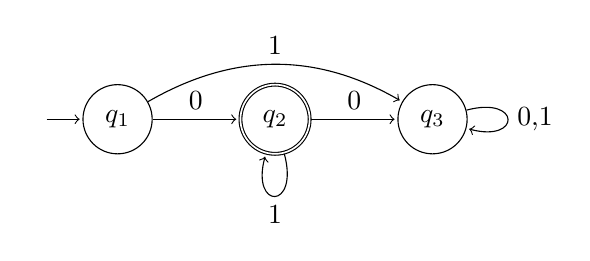
\begin{tikzpicture}[shorten >=1pt, node distance=2cm, on grid, auto]
        \node[state, initial, initial text=] (q1)   {$q_1$};
        \node[state, accepting] (q2) [right=of q1] {$q_2$};
        \node[state] (q3) [right=of q2] {$q_3$};
        
        \path[->]
        (q1) edge [bend left] node {1} (q3)
             edge node {0} (q2)
        (q2) edge [loop below] node {1} ()
             edge node {0} (q3)
        (q3) edge [loop right] node {0,1} ();
         
    \end{tikzpicture}
    \end{center}
    }
    Si identifichi il linguaggio riconosciuto dall'automa.\\[0.1cm]


%\item \textbf{Esercizio 11. (*)}\\
%Si consideri il seguente automa regolare su $\Sigma = \{0,1\}$:
%{
%\small
%\begin{center}
%\begin{tikzpicture}[shorten >=1pt, node distance=2cm, on grid, auto]
%    \node[state, initial, initial text=] (p1)   {$p_1$};
%    \node[state, accepting] (p2) [right=of p1] {$p_2$};
%    \node[state] (p3) [right=of p2] {$p_3$};
%    
%    \path[->]
%    (p1) edge [loop above] node {1} (p1)
%         edge [bend left] node {0} (p2)
%    (p2) edge [loop above] node {0} (p2)
%         edge [bend left] node {1} (p1)
%         edge [bend left] node {1} (p3)
%    (p3) edge [loop above] node {1} (p3)
%         edge [bend left] node {0} (p2)
%    
%\end{tikzpicture}
%\end{center}
%}
%Si identifichi il linguaggio riconosciuto dall'automa.


    \item \textbf{Esercizio 17. (**)}\\
    Si consideri il seguente automa regolare su $\Sigma = \{a,b,c\}$:
    {
    \small
    \begin{center}
    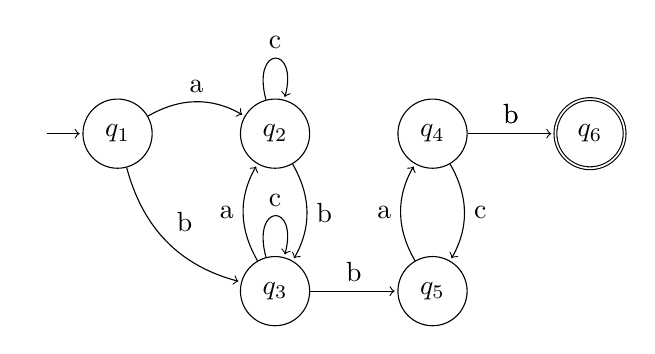
\begin{tikzpicture}[shorten >=1pt, node distance=2cm, on grid, auto]
        
        \node[state] (q2) {$q_2$};
        \node[state, below=of q2] (q3) {$q_3$};

        \node[state, right=of q2] (q4) {$q_4$};
        \node[state, below=of q4] (q5) {$q_5$};
        \node[state, right=of q4, accepting] (q6) {$q_6$};

        \node[state, initial, initial text=, left=of q2] (q1) {$q_1$};

        \path[->]
        (q1) edge [bend left] node {a} (q2)
             edge [bend right] node {b} (q3)
        (q2) edge [bend left] node {b} (q3)
             edge [loop above] node {c} ()
        (q3) edge [bend left] node {a} (q2)
             edge [loop above] node {c} ()
             edge node {b} (q5)
        (q5) edge [bend left] node {a} (q4)
        (q4) edge [bend left] node {c} (q5)
             edge node {b} node {b} (q6);

    \end{tikzpicture}
    \end{center}
    }
    Si identifichi il linguaggio riconosciuto dall'automa.
    
\end{itemize}
}
\vfill
\noindent\makebox[\linewidth]{\rule{\linewidth}{0.1pt}}
\end{document}
